\chapter{Estudios experimentales}
\section{Introducción}
Para validar el algoritmo presentado en esta tesis, se adoptó un conjunto de instancias de prueba del FJSSP, otorgando grandes ventajas a la hora de comparar los resultados obtenidos frente a otros algoritmos. A fin de permitir una comparación cuantitativa de resultados, en este trabajo se utilizaron tablas comparativas que exponen los valores óptimos, los mejores obtenidos y las medias de los mismos, junto con el desvío estándar. Además se utilizó el error relativo, que es el cociente entre el error absoluto de una medida y el valor real de ésta, mostrados en forma de gráficos de caja (\textit{boxplot} en inglés), los cuales son una forma de presentación estadística destinada, fundamentalmente, a resaltar aspectos de la distribución de las observaciones en una o más series de datos cuantitativos. El gráfico de caja es una buena alternativa a la presentación tradicional de datos medidos con escala cuantitativa, pues permite cotejar varias series de datos medidas con la misma escala y ubicadas en posiciones parecidas de ésta, siendo, en tal sentido, más claro y de mayor información que otros tipos de gráficos.


Dado que el objetivo del paralelismo es la reducción del tiempo real, se utiliza la aceleración como medida de comparación del algoritmo \textit{DE} frente a su versión paralela. El tiempo debe incluir cualquier actividad que se realice en el proceso, por lo que la opción más prudente para medir el rendimiento de un código paralelo es considerar el tiempo entre el inicio y fin de todo el algoritmo para resolver el problema en cuestión. Para una comparación justa, la misma idea debe ser tomada en consideración en el caso secuencial.


En este capítulo se describe el diseño experimental llevado a cabo para este trabajo. Además se presentan los resultados experimentales obtenidos variando el factor de escalado ($F$) y la probabilidad de recombinación ($Cr$), agregando el procedimiento de búsqueda local y la mejora en tiempo del algoritmo gracias al paralelismo. Por último, se lleva a cabo una comparación de los resultados del algoritmo \textit{HDE} frente a otros algoritmos competitivos presentes en la literatura.

\section{Diseño experimental}


En esta sección, se describe el diseño experimental utilizado en este trabajo. Se selecciona una amplia gama de instancias del FJSSP utilizadas en la literatura teniendo en cuenta su complejidad, que viene dada por el número de trabajos y máquinas, y la amplia variación de flexibilidad en la cantidad de máquinas disponibles por operación. En este sentido, fue considerado el conjunto de datos propuestos por Brandimarte \cite{Brandimarte} presentado en la tabla \ref{tab:InstanciasBrandirmarte}, ya que el número de trabajos varía de 10 a 20, el número de máquinas pertenece al rango [4,15] y el número de operaciones para cada trabajo puede tomar valores desde 5 a 15, en consecuencia, el número total de operaciones va desde 55 a 255. Teniendo en cuenta la flexibilidad esta oscila entre 1.43 y 4.10 \cite{MinettiSalto}.


% Table generated by Excel2LaTeX from sheet 'Hoja 1'
\begin{table}[!tb]
    \scriptsize
  \centering
  \caption{Instancias propuestas por Brandimarte}
    \begin{tabular}{|c|c|c|c|c|}
    \hline
    \textbf{Instancia} & \textbf{Cantidad de trabajos} & \textbf{Cantidad de operaciones} & \textbf{Cantidad de máquinas} & \textbf{Óptimo} \bigstrut\\
    \hline
    Mk01 & 10  & 55  & 6   & 40 \\
    Mk02 & 10  & 58  & 6   & 26 \\
    Mk03 & 15  & 150 & 8   & 204 \\
    Mk04 & 15  & 90  & 8   & 60 \\
    Mk05 & 15  & 106 & 4   & 172 \\
    Mk06 & 10  & 150 & 15  & 58 \\
    Mk07 & 20  & 100 & 5   & 139 \\
    Mk08 & 20  & 255 & 10  & 523 \\
    Mk09 & 20  & 240 & 10  & 307 \\
    Mk10 & 20  & 240 & 15  & 197 \\
    \hline
    \end{tabular}%
  \label{tab:InstanciasBrandirmarte}%
\end{table}%

Con respecto a la metodología seguida para analizar los resultados, primero, estudiamos el comportamiento de estos algoritmos con diferentes valores de $ Cr$ y $F$, considerando los mejores $ C_ {max} $ encontrados y el error relativo de $ C_ {max} $ contra el óptimo conocido en cada instancia. Estos análisis nos permiten determinar los mejores valores para los parámetros de control. En segundo lugar, determinamos el impacto de incorporar un procedimiento de búsqueda local a diferentes probabilidades $ P_ {BL} $. Para este propósito, tomamos en cuenta los mejores $ C_ {max} $ encontrados, la tasa de aciertos (es decir, la cantidad de veces que un algoritmo encuentra la mejor solución) y el error relativo de $ C_ {max} $ contra el óptimo conocido en cada instancia. Finalmente, estudiamos el comportamiento del algoritmo de \textit{DE} híbrido incluyendo el paralelismo con respecto al tiempo de ejecución en cada enfoque.


Los algoritmos considerados fueron programados en C++, por lo que su tiempo de ejecución es directamente comparable. Todos los algoritmos se compilaron en la misma computadora con los mismos indicadores de compilación y se ejecutaron en hardware homogéneo. La experimentación se llevó a cabo en un clúster conformado por cuatro máquinas con INTEL I7 3770K, 8 GB de RAM y el Slackware Linux con la versión 2.6.27 del núcleo. Para implementar la versión paralela de DE, se utiliza una interfaz de programación de aplicaciones (API) para computadoras paralelas de memoria compartida como es OpenMP \cite{openMP}.


\begin{table}[b]
    \scriptsize
\centering
\caption{Valores de los parámetros}
    \begin{tabular}{|c|c|}
    \hline
    \multicolumn{1}{|c|}{\textbf{Parámetro}} & \multicolumn{1}{c|}{\textbf{Valor}} \\ 
    \hline
    $N_P$                              & 50                          \\
    $F$                               & 0.1, 0.5, y 0.9           \\
    $Cr$                              & 0.1, 0.5, y 0.9                 \\
    $P_{BL}$                          & 0.1, 0.5, y 0.7          \\
    \hline
    \end{tabular}
\label{tab:DEparameteres}%
\end{table}


Para este estudio, la configuración paramétrica del DE es la que se muestra en la tabla \ref{tab:DEparameteres}. El tamaño de la población, $ N_P $, fue adoptado de trabajos anteriores y se establece en 50. Con respecto a la probabilidad de $Cr$ y el factor $F$, se consideraron tres valores diferentes para cada uno de ellos 0.1, 0.5 y 0.9.
Utilizar un valor de $Cr$ alto implica que el vector prueba hereda muchos componentes del vector donador. En caso contrario, si es muy bajo, el vector prueba hereda muchos componentes del vector objetivo. Un valor intermedio como el de 0.5, produciría una situación intermedia e incrementaría la diversidad poblacional. Los valores extremos harían que la diversidad poblacional no fuese incrementada.
El factor de escalado $F$ controla la longitud del salto generado en la explotación del espacio de búsqueda. Un valor bajo lleva al algoritmo a intensificar la explotación de soluciones en algunas regiones del espacio de búsqueda, mientras que un valor alto implica una mayor diversificacion de las soluciones, explorando en mayor medida todo el espacio de búsqueda. Un valor intermedio hace un balance entre diversificación e intensificación.
Para el parámetro restante, $ P_{BL} $, también se analizaron tres valores 0.1, 0.5 y 0.7 (valores con baja, media y alta probabilidad), para estudiar cómo la frecuencia de aplicación de la búsqueda local impacta en los resultados arrojados por el \textit{DE}.


Para hacer una comparación justa entre estos algoritmos, deben hacer el mismo esfuerzo computacional en cada ejecución. Puede lograrse si se ejecuta durante el mismo tiempo cada instancia del problema. De esta manera, el tiempo total ejecutado para una instancia se calcula teniendo en cuenta su tamaño. En la Ecuación \ref{eqtime2} se explica cómo se calcula el tiempo total de ejecución, donde $\sharp O $ es el cantidad de operaciones para una instancia determinada.

\begin{equation}\label{eqtime2}
TiempoEjecucion = \sharp O \times (\frac{\sharp O}{2})\times 30 
\end{equation}

Debido a la naturaleza estocástica de los algoritmos, fueron realizadas 30 ejecuciones independientes de cada prueba con el fin de recopilar datos experimentales significativos y aplicar métricas de confianza estadística para validar las conclusiones.


\section{Resultados experimentales}

En esta sección, analizamos la calidad de los resultados considerando los valores de $ C_ {max} $ obtenidos para las distintas mejoras planteadas al algoritmo DE descrito en el capítulo anterior para resolver las instancias de FJSSP.
En primer lugar se estudiará la influencia de los parámetros $Cr$ y $F$, luego la incorporación del proceso de búsqueda local a través del parámetro $P_{BL}$, después el impacto en los tiempos al incorporar un paralelismo a nivel de iteración y por último se hace una comparación de los valores de $ C_ {max} $ obtenidos por el algoritmo con los alcanzados por varios algoritmos competitivos presentes en la literatura. 


\subsection{Resultados variando los parámetros $F$ y $Cr$ }

El primer análisis se centra en el efecto de usar diferentes valores de $F$ y $Cr$ en el rendimiento de \textit{DE}, de valores bajos a altos (0.1, 0.5 y 0.9). Para este fin, se analizó la calidad de los resultados teniendo en cuenta los valores de $C_{max}$ obtenidos para el \textit{DE} básico al resolver las instancias FJSSP, es decir, se estudió cómo impacta en el rendimiento de \textit{DE} el utilizar las distintas combinaciones de valores de parámetros.


La tabla \ref{tab:resultadosDE} muestra los mejores valores de $C_{max}$ obtenidos para el \textit{DE} utilizando las combinaciones posibles de valores de $F$ y $Cr$ para cada instancia. La columna 2 presenta el mejor valor conocido de $C_{max}$ (óptimo) para cada instancia. La última fila de esta tabla muestra la relación entre el número de instancias resueltas de forma óptima con respecto al número total de instancias. En la tabla \ref{tab:resultadosDEmedias} se encuentran los valores medios de $C_{max}$ junto con la desviación estándar media para los distintos valores de $F$ y $Cr$. 


\begin{table}[t]
    \scriptsize
  \centering
  \caption{Mejores valores de $C_{max}$ encontrados por el \textit{DE} con diferentes valores de $F$ y $Cr$ para todas las instancias del FJSSP}
    \begin{tabular}{|rrccccccccc|}
    \hline
    \multicolumn{1}{|c|}{\multirow{}} & \multicolumn{1}{c|}{\multirow{}} & \multicolumn{9}{c|}{\textbf{Mejor valor de C_{max}}} \bigstrut\\
\cline{3-11}    \multicolumn{1}{|c|}{{\textbf{Instancia}}} & \multicolumn{1}{c|}{{\textbf{Opt.}}} & \multicolumn{1}{c|}{\textbf{F=0.1}} & \multicolumn{1}{c|}{\textbf{F=0.1}} & \multicolumn{1}{c|}{\textbf{F=0.1}} & \multicolumn{1}{c|}{\textbf{F=0.5}} & \multicolumn{1}{c|}{\textbf{F=0.5}} & \multicolumn{1}{c|}{\textbf{F=0.5}} & \multicolumn{1}{c|}{\textbf{F=0.9}} & \multicolumn{1}{c|}{\textbf{F=0.9}} & \multicolumn{1}{c|}{\textbf{F=0.9}} \\
    \multicolumn{1}{|c|}{} & \multicolumn{1}{c|}{} & \multicolumn{1}{c|}{\textbf{Cr=0.1}} & \multicolumn{1}{c|}{\textbf{Cr=0.5}} & \multicolumn{1}{c|}{\textbf{Cr=0.9}} & \multicolumn{1}{c|}{\textbf{Cr=0.1}} & \multicolumn{1}{c|}{\textbf{Cr=0.5}} & \multicolumn{1}{c|}{\textbf{Cr=0.9}} & \multicolumn{1}{c|}{\textbf{Cr=0.1}} & \multicolumn{1}{c|}{\textbf{Cr=0.5}} & \multicolumn{1}{c|}{\textbf{Cr=0.9}} \\
    \hline
    \multicolumn{1}{|c|}{Mk01} & \multicolumn{1}{c|}{40} & \multicolumn{1}{c|}{\textbf{40}} & \multicolumn{1}{c|}{\textbf{40}} & \multicolumn{1}{c|}{\textbf{40}} & \multicolumn{1}{c|}{\textbf{40}} & \multicolumn{1}{c|}{\textbf{40}} & \multicolumn{1}{c|}{\textbf{40}} & \multicolumn{1}{c|}{\textbf{40}} & \multicolumn{1}{c|}{\textbf{40}} & \textbf{40} \bigstrut\\
    %\hline
    \multicolumn{1}{|c|}{Mk02} & \multicolumn{1}{c|}{26} & \multicolumn{1}{c|}{\textbf{26}} & \multicolumn{1}{c|}{27} & \multicolumn{1}{c|}{27} & \multicolumn{1}{c|}{\textbf{26}} & \multicolumn{1}{c|}{27} & \multicolumn{1}{c|}{\textbf{26}} & \multicolumn{1}{c|}{27} & \multicolumn{1}{c|}{27} & 27 \bigstrut\\
    %\hline
    \multicolumn{1}{|c|}{Mk03} & \multicolumn{1}{c|}{204} & \multicolumn{1}{c|}{\textbf{204}} & \multicolumn{1}{c|}{\textbf{204}} & \multicolumn{1}{c|}{\textbf{204}} & \multicolumn{1}{c|}{\textbf{204}} & \multicolumn{1}{c|}{\textbf{204}} & \multicolumn{1}{c|}{\textbf{204}} & \multicolumn{1}{c|}{\textbf{204}} & \multicolumn{1}{c|}{\textbf{204}} & \textbf{204} \bigstrut\\
    %\hline
    \multicolumn{1}{|c|}{Mk04} & \multicolumn{1}{c|}{60} & \multicolumn{1}{c|}{\textbf{60}} & \multicolumn{1}{c|}{\textbf{60}} & \multicolumn{1}{c|}{65} & \multicolumn{1}{c|}{61} & \multicolumn{1}{c|}{\textbf{60}} & \multicolumn{1}{c|}{\textbf{60}} & \multicolumn{1}{c|}{62} & \multicolumn{1}{c|}{63} & 62 \bigstrut\\
    %\hline
    \multicolumn{1}{|c|}{Mk05} & \multicolumn{1}{c|}{172} & \multicolumn{1}{c|}{175} & \multicolumn{1}{c|}{173} & \multicolumn{1}{c|}{173} & \multicolumn{1}{c|}{175} & \multicolumn{1}{c|}{179} & \multicolumn{1}{c|}{173} & \multicolumn{1}{c|}{175} & \multicolumn{1}{c|}{179} & 173 \bigstrut\\
    %\hline
    \multicolumn{1}{|c|}{Mk06} & \multicolumn{1}{c|}{58} & \multicolumn{1}{c|}{65} & \multicolumn{1}{c|}{59} & \multicolumn{1}{c|}{63} & \multicolumn{1}{c|}{66} & \multicolumn{1}{c|}{69} & \multicolumn{1}{c|}{59} & \multicolumn{1}{c|}{67} & \multicolumn{1}{c|}{70} & 61 \bigstrut\\
    %\hline
    \multicolumn{1}{|c|}{Mk07} & \multicolumn{1}{c|}{139} & \multicolumn{1}{c|}{143} & \multicolumn{1}{c|}{140} & \multicolumn{1}{c|}{142} & \multicolumn{1}{c|}{143} & \multicolumn{1}{c|}{148} & \multicolumn{1}{c|}{140} & \multicolumn{1}{c|}{144} & \multicolumn{1}{c|}{146} & 140 \bigstrut\\
    %\hline
    \multicolumn{1}{|c|}{Mk08} & \multicolumn{1}{c|}{523} & \multicolumn{1}{c|}{\textbf{523}} & \multicolumn{1}{c|}{\textbf{523}} & \multicolumn{1}{c|}{\textbf{523}} & \multicolumn{1}{c|}{\textbf{523}} & \multicolumn{1}{c|}{\textbf{523}} & \multicolumn{1}{c|}{\textbf{523}} & \multicolumn{1}{c|}{\textbf{523}} & \multicolumn{1}{c|}{\textbf{523}} & \textbf{523} \bigstrut\\
    %\hline
    \multicolumn{1}{|c|}{Mk09} & \multicolumn{1}{c|}{307} & \multicolumn{1}{c|}{318} & \multicolumn{1}{c|}{\textbf{307}} & \multicolumn{1}{c|}{310} & \multicolumn{1}{c|}{321} & \multicolumn{1}{c|}{333} & \multicolumn{1}{c|}{\textbf{307}} & \multicolumn{1}{c|}{321} & \multicolumn{1}{c|}{338} & \textbf{307} \bigstrut\\
    %\hline
    \multicolumn{1}{|c|}{Mk10} & \multicolumn{1}{c|}{197} & \multicolumn{1}{c|}{237} & \multicolumn{1}{c|}{210} & \multicolumn{1}{c|}{221} & \multicolumn{1}{c|}{238} & \multicolumn{1}{c|}{245} & \multicolumn{1}{c|}{206} & \multicolumn{1}{c|}{240} & \multicolumn{1}{c|}{246} & 215 \bigstrut\\
    \hline
        &     & 5/10 & 5/10 & 3/10 & 4/10 & 4/10 & 6/10 & 3/10 & 3/10 & 4/10 \bigstrut\\
    \hline
    \end{tabular}%
\label{tab:resultadosDE}
\end{table}%

% Table generated by Excel2LaTeX from sheet 'DE media y sd'

\begin{table}[!tb]
   \scriptsize
  \centering
  \caption{Valores medios de $C_{max}$ encontrados por el \textit{DE} con diferentes valores de $F$ y $Cr$ para todas las instancias del FJSSP}
    \begin{adjustbox}{max width=\textwidth}
    \begin{tabular}{|c|c|c|c|c|c|c|c|c|c|}
    \hline
    \multirow{} & \multicolumn{9}{c|}{\textbf{Valor medio de Cmax y desvío estándar medio }} \\
\cline{2-10}   \textbf{Instancia}     & \multicolumn{1}{c|}{\textbf{F=0,1}} & \multicolumn{1}{c|}{\textbf{F=0.1}} & \multicolumn{1}{c|}{\textbf{F=0.1}} & \multicolumn{1}{c|}{\textbf{F=0.5}} & \multicolumn{1}{c|}{\textbf{F=0.5}} & \multicolumn{1}{c|}{\textbf{F=0.5}} & \multicolumn{1}{c|}{\textbf{F=0.9}} & \multicolumn{1}{c|}{\textbf{F=0.9}} & \multicolumn{1}{c|}{\textbf{F=0.9}} \\
        & \multicolumn{1}{c|}{\textbf{Cr=0.1}} & \multicolumn{1}{c|}{\textbf{Cr=0.5}} & \multicolumn{1}{c|}{\textbf{Cr=0.9}} & \multicolumn{1}{c|}{\textbf{Cr=0.1}} & \multicolumn{1}{c|}{\textbf{Cr=0.5}} & \multicolumn{1}{c|}{\textbf{Cr=0.9}} & \multicolumn{1}{c|}{\textbf{Cr=0.1}} & \multicolumn{1}{c|}{\textbf{Cr=0.5}} & \multicolumn{1}{c|}{\textbf{Cr=0.9}} \bigstrut\\
    \hline
    Mk01 & 40 $_{\pm  0.00}$ & 40.26$_{\pm 0.69 }$& 41.8$_{\pm 0.48 }$& 40$_{\pm 0.00 & 4}$0$_{\pm 0.00 & 4}$0.06$_{\pm 0.25 }$& 40$_{\pm 0.00 & 4}$0.03$_{\pm 0.18 }$& 40.53$_{\pm 0.73 }$\bigstrut\\
    %\hline
    Mk02 & 26.57 $_{\pm  0.50}$ & 27$_{\pm 0.00 & 2}$7.8$_{\pm 0.48 }$& 26.96$_{\pm 0.18 }$& 27.33$_{\pm 0.47 }$& 26.96$_{\pm 0.18 }$& 27.03$_{\pm 0.18 }$& 27.23$_{\pm 0.43 }$& 27.33$_{\pm 0.47 }$\bigstrut\\
    %\hline
    Mk03 & 204 $_{\pm  0.00}$ & 204$_{\pm 0.00 & 2}$04$_{\pm 0.00 & 2}$04$_{\pm 0.00 & 2}$04$_{\pm 0.00 & 2}$04$_{\pm 0.00 & 2}$04$_{\pm 0.00 & 2}$04$_{\pm 0.00 & 2}$04$_{\pm 0.00}$\bigstrut\\
    %\hline
    Mk04 & 60 $_{\pm  0.00}$ & 62.03$_{\pm 1.42 }$& 66.93$_{\pm 0.82 }$& 62.16$_{\pm 0.53 }$& 65.76$_{\pm 1.27 }$& 64.56$_{\pm 1.90 }$& 63.76$_{\pm 0.97 }$& 66.23$_{\pm 0.81 }$& 65.33$_{\pm 1.72 }$\bigstrut\\
    %\hline
    Mk05 & 176.33 $_{\pm  0.66}$ & 177.2$_{\pm 1.67 }$& 175.8$_{\pm 1.07 }$& 176.5$_{\pm 0.73 }$& 181.3$_{\pm 0.96 }$& 173.6$_{\pm 0.92 }$& 176.8$_{\pm 0.69 }$& 181.2$_{\pm 1.01 }$& 173.7$_{\pm 0.94 }$\bigstrut\\
    %\hline
    Mk06 & 66.7 $_{\pm 0.75 }$& 64.2$_{\pm 2.52 }$& 66.13$_{\pm 1.04 }$& 67.53$_{\pm 0.62 }$& 70.83$_{\pm 0.69 }$& 61.93$_{\pm 1.36 }$& 67.96$_{\pm 0.55 }$& 71.1$_{\pm 0.54 }$& 63.53$_{\pm 1.19 }$\bigstrut\\
    %\hline
    Mk07 & 144.3 $_{\pm  0.53}$ & 143.8$_{\pm 2.02 }$& 144.5$_{\pm 1.27 }$& 144.5$_{\pm 0.77 }$& 150.1$_{\pm 0.94 }$& 141.8$_{\pm 1.39 }$& 144.8$_{\pm 0.79 }$& 150.1$_{\pm 1.11 }$& 142.1$_{\pm 1.12 }$\bigstrut\\
    %\hline
    Mk08 & 523 $_{\pm  0.00}$ & 523$_{\pm 0.00 & 5}$23$_{\pm 0.00 & 5}$23$_{\pm 0.00 & 5}$23.5$_{\pm 1.04 }$& 523$_{\pm 0.00 & 5}$23$_{\pm 0.00 & 5}$23.6$_{\pm 0.95 }$& 523$_{\pm 0.00}$\bigstrut\\
    %\hline
    Mk09 & 323.6 $_{\pm  2.44}$ & 316.1$_{\pm 7.98 }$& 323.9$_{\pm 6.23 }$& 326.3$_{\pm 2.35 }$& 341.5$_{\pm 2.87 }$& 307.5$_{\pm 1.47 }$& 327.9$_{\pm 2.32 }$& 342.3$_{\pm 2.29 }$& 310.7$_{\pm 3.46 }$\bigstrut\\
    %\hline
    Mk10 & 240.63 $_{\pm  1.54}$ & 239.5$_{\pm 7.10 }$& 226.8$_{\pm 2.83 }$& 242.1$_{\pm 1.85 }$& 251.2$_{\pm 2.12 }$& 212.4$_{\pm 2.99 }$& 242.3$_{\pm 1.32 }$& 251.7$_{\pm 1.86 }$& 219.5$_{\pm 2.66 }$\bigstrut\\
    \hline
    \end{tabular}%
    \end{adjustbox}
\label{tab:resultadosDEmedias}
\end{table}%

Como se puede ver en la Tabla \ref{tab:resultadosDE},  el \textit{DE} encuentra el óptimo en 3 instancias (MK01, MK03 y MK08) independientemente de las combinaciones de valores de $F$ y $Cr$ consideradas. Con un valor alto de $F$ \textit{DE} tiene menos posibilidades de encontrar las mejores soluciones para el FJSSP sin importar el valor de $Cr$ usado, ya que la cantidad de valores óptimos alcanzados para las diferentes instancias es menor frente a otras posibles combinaciones de valores paramétricos (no más de 4 de las 10 instancias). El \textit{DE} con $F = 0.5 $ y $Cr = 0.9 $ encuentra una mayor cantidad de veces valores de $ C_ {max} $ óptimos que el resto de las combinaciones (en 6 de las 10 instancias).


Una métrica importante es el error relativo de los mejores $ C_ {max} $ obtenidos para cada instancia con respecto al óptimo. Esta métrica nos permite normalizar los datos de las diferentes instancias y, de esta manera, enfocar la atención en cómo las diferentes combinaciones de valores de $F$ y $Cr$ afectan al rendimiento de \textit{DE} al resolver el FJSSP. Observando el \textit{boxplot} del error relativo para las distintas combinaciones de parámetros de $F$ y $Cr$ presentado en la Figura \ref{fig:DEboxplot} se puede ver que el algoritmo \textit{DE} con $F = 0.5 $ y $Cr = 0.9 $ presenta la menor mediana del error. La caja de rango intercuartil muestra que la distancia entre el primer cuartil y el tercer cuartil es menor frente a otras posibles combinaciones de valores de parámetros. Los bigotes que se extienden desde la parte superior de la caja son claramente inferiores frente a los de las demás combinaciones. Por último, se puede observar que no existen valores atípicos, lo cual presenta una superioridad con respecto a las posibles elecciones de parámetros. 

\begin{figure}[H]
   \scriptsize
    \centering
    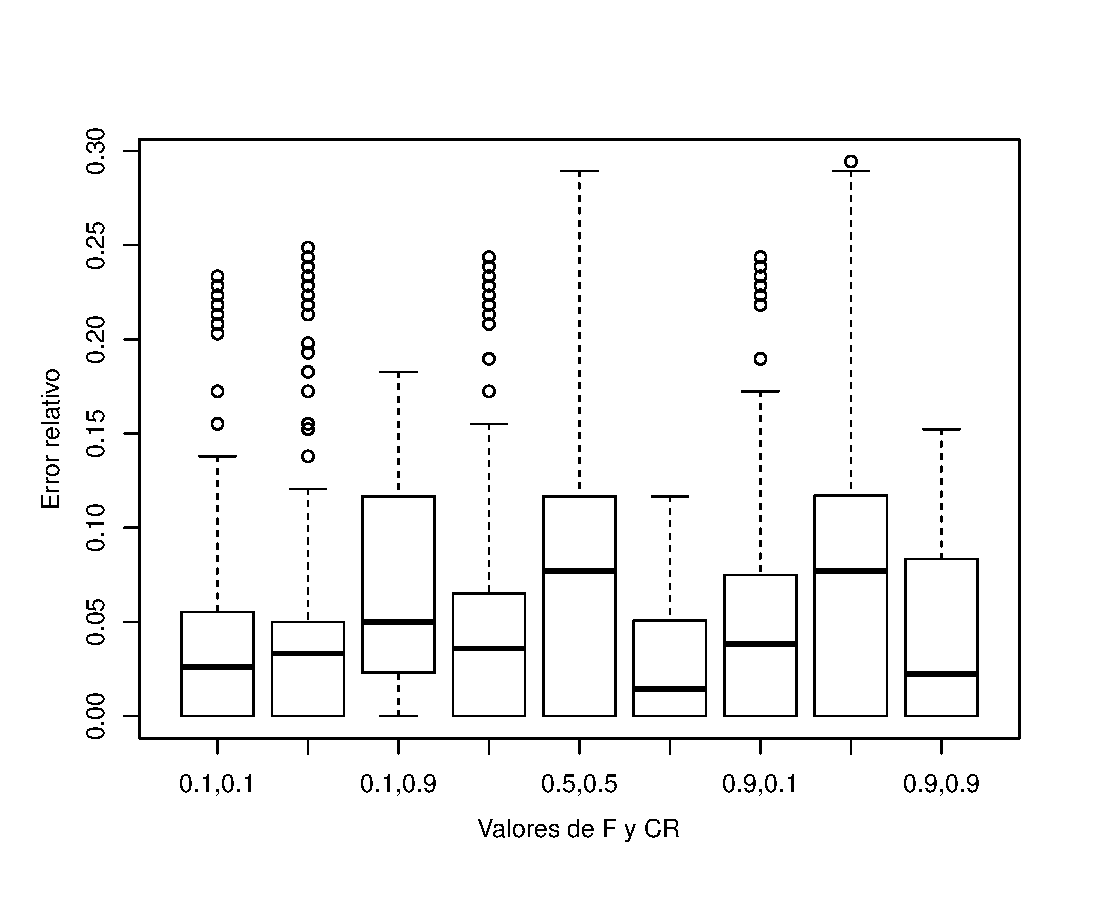
\includegraphics[trim={0 1cm 0 0.8cm},scale=0.6]{images/Boxplot-DE.eps}
    \caption{Boxplot del error relativo del \textit{DE} para distintos valores de $F$ y $Cr$.}
    \label{fig:DEboxplot}
\end{figure}


Finalmente, se estudiará la distribución del número de evaluaciones realizadas por \textit{DE} para encontrar los mejores valores de $ C_ {max} $ para las diferentes combinaciones de $F$ y $Cr$. Con este fin, la Figura \ref{fig:DE10boxplot} ilustra los resultados utilizando diez \textit{boxplots} (uno por cada instancia). En general, se observa que el algoritmo \textit{DE} con menor cantidad de evaluaciones es aquel con $F\in \{0.1,0.5\}$ y $Cr=0.9$, pero la combinación $F = 0.5 $ y $Cr = 0.9 $ supera a las demás desde el punto de vista de la calidad de resultados (ver Tabla \ref{tab:resultadosDE}). En consecuencia, serán considerados los valores de $F = 0.5 $ y $Cr = 0.9 $ en la experimentación restante.

\begin{figure}[H]
   \scriptsize
    \centering
    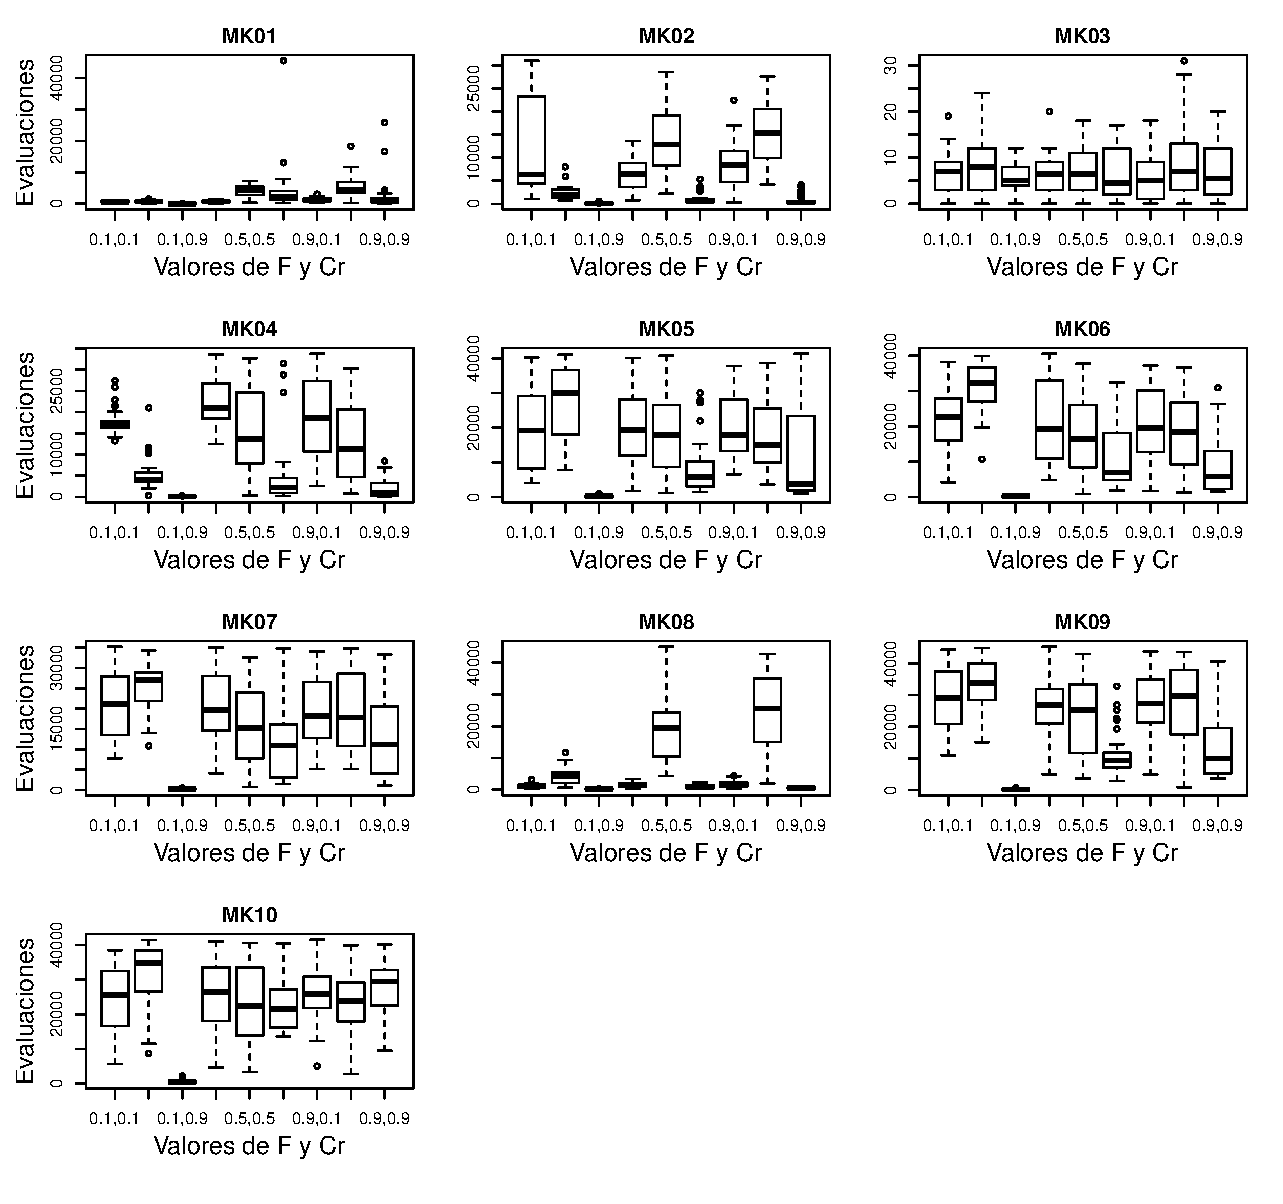
\includegraphics[trim={0 0.6cm 0 0cm},scale=0.7]{images/DE-10boxplot.eps}
    \caption{Boxplot del error relativo del \textit{DE} para distintos valores de $F$ y $Cr$.}
    \label{fig:DE10boxplot}
\end{figure}


\subsection{Resultados de \textit{DE} con búsqueda local}
En esta sub-sección se analiza en detalle lo que sucede al introducir un procedimiento de búsqueda local en el algoritmo \textit{DE} para resolver las instancias de FJSSP. El algoritmo resultante es llamado \textit{HDE}. Para esos estudios, fueron considerados tres valores diferentes de $P_{BL}$: 0.1, 0.5 y 0.7 (de valores altos a bajos), es decir, se estudió cómo la frecuencia de la aplicación del procedimiento de búsqueda local impacta en el rendimiento de \textit{HDE}.


La tabla \ref{tab:tableDELS} muestra los mejores y la media de los valores de $C_{max}$ obtenidos para el algoritmo \textit{HDE} con los diferentes valores de $P_{BL}$. El algoritmo \textit{HDE} obtiene un número mayor de $C_{max}$ óptimos con $P_{BL} = 0.5$ y con $P_{BL} = 0.7$. Pero el algoritmo \textit{HDE} que aplica el procedimiento de búsqueda local con la frecuencia más alta ($P_{BL} = 0.7$) presenta valores de $C_{max}$ medios más bajo para todas las instancias. Esto indica que el algoritmo encuentra el valor óptimo o casi óptimo en la mayoría de las ejecuciones, lo cual queda claramente plasmado en el \textit{boxplot} del error relativo de las distintas instancias contra los óptimos para los distintos valores de $P_{BL}$ presentado en la figura ~\ref{fig:DELSboxplot}, donde se observa que la mediana del error es menor con la frecuencia de búsqueda local más alta.


% Table generated by Excel2LaTeX from sheet 'Hoja1'
\begin{table}[!tb]
  \centering
     \scriptsize
    \caption{Valores de $C_{max}$ encontrados por el \textit{HDE} con diferentes valores de $P_{BL}$ para todas las instancias de FJSSP.}
    \begin{tabular}{|rrcccrrc|}
    \hline
    \multicolumn{1}{|c|}{\multirow{}{\textbf{Instancia}}} & \multicolumn{1}{c|}{\multirow{}{\textbf{Optimos}}} & \multicolumn{3}{c|}{\textbf{Mejor valor de Cmax}} & \multicolumn{3}{c|}{\textbf{Valor medio de Cmax y desvío estándar medio }} \bigstrut\\
\cline{3-8}    \multicolumn{1}{|c|}{} & \multicolumn{1}{c|}{} & \multicolumn{1}{c|}{\textbf{$P_{BL}=0.1$}} & \multicolumn{1}{c|}{\textbf{$P_{BL}=0.5$}} & \multicolumn{1}{c|}{\textbf{$P_{BL}=0.7$}} & \multicolumn{1}{c|}{\textbf{$P_{BL}=0.1$}} & \multicolumn{1}{c|}{\textbf{$P_{BL}=0.5$}} & \multicolumn{1}{c|}{\textbf{$P_{BL}=0.7$}} \bigstrut\\
    \hline
    \multicolumn{1}{|c|}{Mk01} & \multicolumn{1}{c|}{40} & \multicolumn{1}{c|}{\textbf{40}} & \multicolumn{1}{c|}{\textbf{40}} & \multicolumn{1}{c|}{\textbf{40}} & \multicolumn{1}{c|}{40$_{\pm 0.00}$} & \multicolumn{1}{c|}{40$_{\pm 0.00}$} & 40$_{\pm 0.00}$ \bigstrut\\
    %\hline
    \multicolumn{1}{|c|}{Mk02} & \multicolumn{1}{c|}{26} & \multicolumn{1}{c|}{27} & \multicolumn{1}{c|}{\textbf{26}} & \multicolumn{1}{c|}{\textbf{26}} & \multicolumn{1}{c|}{27.03$_{\pm 0.18}$} & \multicolumn{1}{c|}{26.96$_{\pm 0.18}$} & 26.76$_{\pm 0.43}$ \bigstrut\\
    %\hline
    \multicolumn{1}{|c|}{Mk03} & \multicolumn{1}{c|}{204} & \multicolumn{1}{c|}{\textbf{204}} & \multicolumn{1}{c|}{\textbf{204}} & \multicolumn{1}{c|}{\textbf{204}} & \multicolumn{1}{c|}{204$_{\pm 0.00}$} & \multicolumn{1}{c|}{204$_{\pm 0.00}$} & 204$_{\pm 0.00}$ \bigstrut\\
    %\hline
    \multicolumn{1}{|c|}{Mk04} & \multicolumn{1}{c|}{60} & \multicolumn{1}{c|}{\textbf{60}} & \multicolumn{1}{c|}{\textbf{60}} & \multicolumn{1}{c|}{\textbf{60}} & \multicolumn{1}{c|}{62$_{\pm 1.31}$} & \multicolumn{1}{c|}{61.3$_{\pm 0.70}$} & 61.03$_{\pm 0.66}$ \bigstrut\\
    %\hline
    \multicolumn{1}{|c|}{Mk05} & \multicolumn{1}{c|}{172} & \multicolumn{1}{c|}{173} & \multicolumn{1}{c|}{173} & \multicolumn{1}{c|}{173} & \multicolumn{1}{c|}{174.3$_{\pm 0.75}$} & \multicolumn{1}{c|}{173$_{\pm 0.00}$ }& 173$_{\pm 0.00}$ \bigstrut\\
    %\hline
    \multicolumn{1}{|c|}{Mk06} & \multicolumn{1}{c|}{58} & \multicolumn{1}{c|}{63} & \multicolumn{1}{c|}{62} & \multicolumn{1}{c|}{61} & \multicolumn{1}{c|}{64.4$_{\pm 0.56}$} & \multicolumn{1}{c|}{62.83$_{\pm 0.53}$} & 62.43$_{\pm 0.62}$ \bigstrut\\
    %\hline
    \multicolumn{1}{|c|}{Mk07} & \multicolumn{1}{c|}{139} & \multicolumn{1}{c|}{142} & \multicolumn{1}{c|}{140} & \multicolumn{1}{c|}{140} & \multicolumn{1}{c|}{143.2$_{\pm 0.69}$} & \multicolumn{1}{c|}{142.0$_{\pm 0.90}$} & 141.8$_{\pm 0.92}$ \bigstrut\\
    %\hline
    \multicolumn{1}{|c|}{Mk08} & \multicolumn{1}{c|}{523} & \multicolumn{1}{c|}{\textbf{523}} & \multicolumn{1}{c|}{\textbf{523}} & \multicolumn{1}{c|}{\textbf{523}} & \multicolumn{1}{c|}{523$_{\pm 0.00}$} & \multicolumn{1}{c|}{523$_{\pm 0.00}$} & 523$_{\pm 0.00}$ \bigstrut\\
    %\hline
    \multicolumn{1}{|c|}{Mk09} & \multicolumn{1}{c|}{307} & \multicolumn{1}{c|}{309} & \multicolumn{1}{c|}{\textbf{307}} & \multicolumn{1}{c|}{\textbf{307}} & \multicolumn{1}{c|}{313.1$_{\pm 2.20}$} & \multicolumn{1}{c|}{310.0$_{\pm 1.33}$} & 309.0$_{\pm 1.72}$ \bigstrut\\
    %\hline
    \multicolumn{1}{|c|}{Mk10} & \multicolumn{1}{c|}{197} & \multicolumn{1}{c|}{226} & \multicolumn{1}{c|}{225} & \multicolumn{1}{c|}{224} & \multicolumn{1}{c|}{231.1$_{\pm 2.41}$} & \multicolumn{1}{c|}{228.0$_{\pm 1.36}$} & 227.2$_{\pm 1.38}$ \bigstrut\\
    \hline
          &       & 4/10  & 6/10  & 6/10  &       &       &  \bigstrut\\
    \hline
    \end{tabular}%
    \label{tab:tableDELS}
\end{table}%


Para determinar que el \textit{HDE} presenta una mejora en los valores de $C_{max}$ obtenidos por el \textit{DE}, se realiza una comparación de los valores de los errores relativos mostrados en la Figura \ref{fig:DEboxplot} y los encontrados en la Figura \ref{fig:DELSboxplot}. Se observa que el algoritmo \textit{HDE} con $P_{BL} = 0.7$ presenta menor error relativo frente a los otros presentados en \textit{DE}, lo que indica la ventaja de incorporar la búsqueda local dentro del marco de \textit{DE}.


\begin{figure}[H]
    \centering
    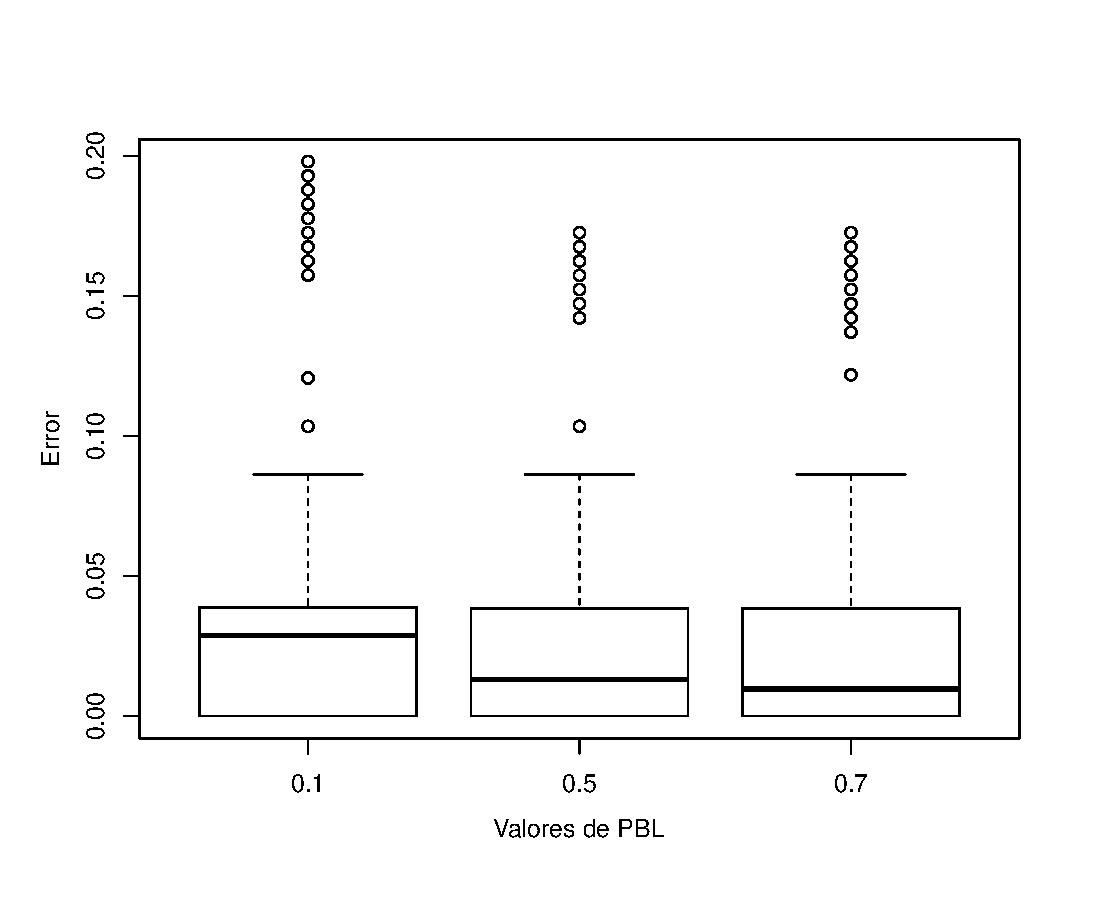
\includegraphics[trim={0 1cm 0 0.8cm},scale=0.6]{images/Boxplot-DELS.eps}
    \caption{Boxplot del error relativo del \textit{HDE} para distintos valores de $P_{BL}$.}
    \label{fig:DELSboxplot}
\end{figure}


\subsection{Resultados de \textit{HDE} y su paralelismo}

En esta subsección se compara el \textit{HDE} contra su versión paralela. La medida más importante de un algoritmo paralelo es el \textit{speedup}. El \textit{speedup} se define como la relación entre el tiempo de ejecución secuencial (tiempo de ejecución de \textit{HDE}, en este caso) y el tiempo de ejecución paralelo. Para este análisis, fue considerado el \textit{speedup} débil \cite{albaMeta2005}. Por esa razón y siguiendo las mejores prácticas de Luque y Alba \cite{LuqueAlba}, el criterio de detención se basa en la calidad de la solución final lograda por los algoritmos, que se establece en los mejores $C_{max}$ conocidos para cada instancia de FJSSP (consulte la columna óptimo de la tabla \ref{tab:InstanciasBrandirmarte}). En consecuencia, los valores de \textit{speedup} solo se informan para las instancias para las cuales el algoritmo \textit{HDE} obtiene el valor óptimo.

 
Una vez establecidos los tiempos de ejecución del algoritmo \textit{HDE} y el algoritmo \textit{HDE} paralelo, se calculan los valores de \textit{speedup}. La Figura \ref{fig:speedup} muestra que el uso de la paralelización vale la pena, ya que permite acelerar el tiempo de ejecución con respecto al \textit{HDE} secuencial sobre todas las instancias en un valor de 3 veces en promedio. El valor ideal de aceleración es 4, el número de núcleos disponibles por máquina, logrando así una aceleración lineal.


\begin{figure}[H]
    \centering
    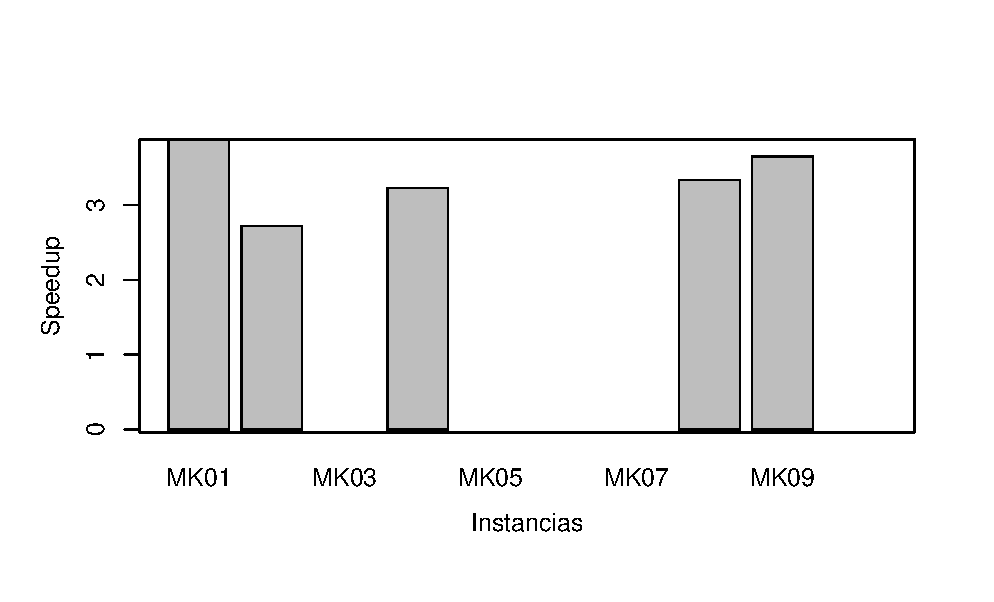
\includegraphics[trim={0 1cm 0 0.7cm},scale=0.7]{images/speedup.eps}
    \caption{\textit{Speedup} por instancia del FJSSP.}
    \label{fig:speedup}
\end{figure}

\section{Comparación de \textit{HDE} con la literatura}

Finalmente, se presenta una comparación de los valores de $C_{max}$ obtenidos por el \textit{HDE} con los alcanzados por varios algoritmos competitivos presentes en la literatura destinados a resolver el FJSSP. Esto permite determinar qué tan buena es la metaheurística presentada en este trabajo. En esta comparación, las metaheurísticas basadas en población para resolver el FJSSP consideradas fueron:

\begin{enumerate}[label=\textit{\roman*})]

\item hGA \cite{tang2011}: un algoritmo híbrido que combina la optimización por enjambre de partículas con un algoritmo genético.

\item BEDA \cite{Wang2012917}: un algoritmo de estimación de distribución basado en bi-poblaciones.

\item IACO \cite{WANG2017}: una optimización basada en colonia de hormigas.

\end{enumerate}

La Tabla \ref{tab:comparison} muestra que los valores de $C_{max}$ obtenidos por el \textit{HDE} son similares a los demás algoritmos para la mayoría de las diez instancias. Esta observación sugiere que el \textit{HDE} propuesto en este trabajo es un algoritmo competitivo para resolver el FJSSP. Las comparaciones con respecto al esfuerzo computacional son difíciles de llevar a cabo porque la mayoría de los trabajos no informan el número de evaluaciones. En consecuencia, la eficiencia relativa de los algoritmos comparados es difícil de contrastar para obtener comparaciones significativas.


\begin{table}[H]
\scriptsize
  \centering
  \caption{Comparación entre \textit{HDE} y metaheurísticas basadas en población de la literatura}
    \begin{tabular}{|l|c|c|c|c|c|c|c|c|c|c|}
    \hline
    \multicolumn{1}{|r}{} & \multicolumn{1}{|l}{MK01} & \multicolumn{1}{|l}{MK02} & \multicolumn{1}{|l}{MK03} & \multicolumn{1}{|l}{MK04} & \multicolumn{1}{|l}{MK05} & \multicolumn{1}{|l}{MK06} & \multicolumn{1}{|l}{MK07} & \multicolumn{1}{|l}{MK08} & \multicolumn{1}{|l}{MK09} & \multicolumn{1}{|l|}{MK10} \\
    \hline
    \textit{HDE}   & \textbf{40} & \textbf{26} & \textbf{204} & \textbf{60} & 173   & 61    & 140   & \textbf{523} & \textbf{307} & 224 \\
    hGA   & \textbf{40} & \textbf{26} & \textbf{204} & 62    & \textbf{172} & 65    & 140   & \textbf{523} & 310   & 214 \\
    BEDA  & \textbf{40} & \textbf{26} & \textbf{204} & \textbf{60} & \textbf{172} & 60    & \textbf{139} & \textbf{523} & \textbf{307} & 206 \\
    IACO  & \textbf{40} & \textbf{26} & \textbf{204} & \textbf{60} & 173   & 60    & 140   & \textbf{523} & \textbf{307} & 208 \\
\hline
    \end{tabular}%
  \label{tab:comparison}%
\end{table}%